\documentclass[11pt,a4paper]{article}

% ── Packages ────────────────────────────────────────────────────────────────
\usepackage[T1]{fontenc}
\usepackage[utf8]{inputenc}
\usepackage{lmodern}
\usepackage{microtype}
\usepackage{geometry}
\geometry{margin=1in}

\usepackage{amsmath,amssymb}
\usepackage{graphicx}
\usepackage{booktabs}
\usepackage{array}
\usepackage{multirow}
\usepackage{xcolor}
\usepackage{listings}
\usepackage{hyperref}
\usepackage{cleveref}
\usepackage{enumitem}
\usepackage{float}
\usepackage{caption}
\usepackage{subcaption}
\usepackage{tikz}
\usetikzlibrary{arrows.meta,positioning,shapes.geometric,fit,backgrounds,calc}
\usepackage{pgfplots}
\pgfplotsset{compat=1.18}

% ── Hyperref colours ─────────────────────────────────────────────────────────
\hypersetup{
  colorlinks=true,
  linkcolor=blue!70!black,
  citecolor=green!50!black,
  urlcolor=blue!70!black,
  pdftitle={AAMP: An Open Protocol for Asynchronous Agent-to-Agent Messaging Across Organizational Boundaries},
  pdfauthor={Ajain Vivek},
}

% ── Code listing style ────────────────────────────────────────────────────────
\definecolor{codebg}{rgb}{0.97,0.97,0.97}
\definecolor{codeframe}{rgb}{0.85,0.85,0.85}
\definecolor{codecomment}{rgb}{0.4,0.5,0.4}
\definecolor{codestring}{rgb}{0.6,0.1,0.1}
\definecolor{codekw}{rgb}{0.1,0.2,0.6}

\lstdefinestyle{aamp}{
  backgroundcolor=\color{codebg},
  frame=single,
  framesep=4pt,
  rulecolor=\color{codeframe},
  basicstyle=\ttfamily\footnotesize,
  keywordstyle=\color{codekw}\bfseries,
  stringstyle=\color{codestring},
  commentstyle=\color{codecomment}\itshape,
  breaklines=true,
  breakatwhitespace=true,
  numbers=left,
  numberstyle=\tiny\color{gray},
  numbersep=6pt,
  tabsize=2,
  captionpos=b,
  xleftmargin=12pt,
}
\lstset{style=aamp}

% ── Title block ───────────────────────────────────────────────────────────────
\title{%
  \textbf{AAMP: An Open Protocol for Asynchronous\\
  Agent-to-Agent Messaging Across Organizational Boundaries}%
  \thanks{Code and specification available at
    \url{https://github.com/brainfish-ai/AAMP}.
    Protocol version 0.1.0.
  }
}

\author{%
  \textbf{Ajain Vivek}\\[4pt]
  \textit{Brainfish AI}\\[2pt]
  \texttt{ajain@brainfish.ai}
}

\date{March 2026}

% ─────────────────────────────────────────────────────────────────────────────
\begin{document}
\maketitle

% ── Abstract ──────────────────────────────────────────────────────────────────
\begin{abstract}
As autonomous AI agents proliferate across independent organizations, the absence of a
standardized, secure, and transport-agnostic inter-agent communication protocol has
become a significant barrier to cross-organizational AI collaboration.
Existing approaches---synchronous HTTP APIs, gRPC, the Model Context Protocol (MCP),
and Google's A2A---either require inbound network ports (precluding sandboxed deployments),
lack cryptographic agent identity, or rely on pre-negotiated bilateral authorization
schemes that do not scale to an open ecosystem of agents.

We present \textbf{AAMP} (Agent-to-Agent Messaging Protocol), an open protocol and
reference implementation enabling \emph{asynchronous, stateful choreography} between
agents operated by different organizations with no pre-established relationship.
AAMP draws on four proven primitives: \emph{Decentralized Identifiers} (DIDs, W3C standard)
for self-sovereign agent identity; \emph{UCAN-inspired capability tokens} for
audience-bound, delegatable, scope-limited authorization; \emph{NATS JetStream} for
durable, federated store-and-forward message delivery; and \emph{Agent Cards} with DID
Document service endpoints for decentralized discovery---an analogue to DNS MX records
in SMTP.

We describe the protocol design, a five-layer stack, six message primitives, five
routing topologies, and a capability-negotiation handshake (PROBE). We present a
reference implementation comprising a TypeScript relay server, a TypeScript SDK, a
Python SDK, and a live cross-organizational demo in which a finance agent (Company A)
delegates a PDF summarization task to a research agent (Company B) through federated
relays, with full cryptographic verification at every hop. We analyze the security model
against a zero-trust threat model and compare AAMP with MCP, Google A2A, gRPC, and raw
HTTP on fourteen protocol dimensions.

\textbf{Keywords:} multi-agent systems, inter-agent communication protocol, decentralized
identity, federated messaging, UCAN, DID, NATS JetStream, asynchronous AI coordination.
\end{abstract}

% ── 1 Introduction ─────────────────────────────────────────────────────────────
\section{Introduction}
\label{sec:intro}

The deployment of autonomous AI agents has moved beyond single-organization sandboxes.
Agents built on LangGraph~\cite{langchain2024}, AutoGen~\cite{wu2023autogen},
CrewAI~\cite{crewai2024}, and LlamaIndex~\cite{llamaindex2024} are increasingly expected
to collaborate across organizational boundaries---a finance agent at Company~A
delegating document research to a specialist agent at Company~B, a customer-service
agent routing escalations to a legal-review agent at an external firm.

This cross-organizational collaboration scenario exposes four fundamental problems
that existing protocols do not solve simultaneously:

\begin{enumerate}[leftmargin=*]
  \item \textbf{The inbound-port problem.} Agents running in containers, Kubernetes
    pods, or cloud functions typically have no inbound network exposure. Synchronous
    HTTP, gRPC, and WebSocket protocols all require the receiving agent to be directly
    reachable---impossible in sandboxed environments.

  \item \textbf{The trust problem.} When two agents from different organizations
    communicate, how does the receiver know the sender is who they claim to be, and
    that they are authorized to invoke a specific capability? OAuth 2.0 solves this
    within a pre-established client-server relationship, but not for ad-hoc
    agent-to-agent contact.

  \item \textbf{The durability problem.} Long-running tasks (LLM inference, data
    pipelines, human-in-the-loop review) do not fit in synchronous HTTP timeouts.
    Webhooks require the caller to also be reachable, and no standard exists for
    checkpointing, retry, or resumption of delegated tasks.

  \item \textbf{The discoverability problem.} Before a task is dispatched, the sender
    needs to know whether the recipient agent supports the requested capability, at
    what cost, and with what latency guarantees---without a centralised registry.
\end{enumerate}

We argue that the email ecosystem, built on SMTP~\cite{rfc5321} in the 1980s, solved
an \emph{identical} set of problems for human message exchange: federated delivery
without bilateral setup, store-and-forward durability, envelope-based routing, and
decentralized MX-record discovery. AAMP applies the same architectural principles to
AI agent communication, replacing DNS MX records with DID Document service endpoints,
DKIM signatures with Ed25519, and MIME with a typed Envelope schema.

\paragraph{Contributions.} This paper makes the following contributions:
\begin{itemize}[leftmargin=*]
  \item A formal protocol specification (AAMP v0.1.0) with a five-layer stack, six
    message primitives, five routing topologies (\S\ref{sec:design}), and a
    capability-negotiation handshake (PROBE).
  \item A working reference implementation: TypeScript relay server (Fastify + NATS),
    TypeScript SDK, and Python SDK (\S\ref{sec:impl}).
  \item A cross-organizational end-to-end demo with full cryptographic verification
    (\S\ref{sec:eval}).
  \item A structured comparison of AAMP against MCP, Google A2A, gRPC, and HTTP on
    fourteen protocol dimensions (\S\ref{sec:related}).
  \item A zero-trust security analysis covering seven threat categories (\S\ref{sec:security}).
\end{itemize}

% ── 2 Background and Related Work ─────────────────────────────────────────────
\section{Background and Related Work}
\label{sec:related}

\subsection{Model Context Protocol (MCP)}

MCP~\cite{anthropic2024mcp} by Anthropic defines a standard for connecting AI agents
to \emph{tools and data sources} (databases, APIs, file systems). Its primary
abstraction is agent-to-tool, not agent-to-agent. MCP lacks agent identity, cross-company
federation, and asynchronous task threading. It requires the tool server to expose
inbound SSE or stdio connections. AAMP is designed to sit \emph{above} MCP: an AAMP
agent can use MCP tools internally; AAMP handles the inter-agent coordination layer.

\subsection{Google Agent-to-Agent (A2A)}

Google's A2A protocol~\cite{googlea2a2025} (April 2025) is the closest prior work to
AAMP. It correctly identifies the need for asynchronous task primitives, task lifecycle
management, and Agent Cards for discovery. However, A2A uses OAuth~2.0 for
authorization, which requires Company~A to pre-register an OAuth client with Company~B's
authorization server---a bilateral setup that does not scale to a world of thousands
of independent agents. A2A also requires the receiving agent to expose inbound HTTPS
endpoints and lacks cryptographic agent identity (relying on HTTPS client certificates
rather than self-sovereign DIDs).

\subsection{Decentralized Identifiers and UCAN}

The W3C DID specification~\cite{w3cdid2022} defines a globally unique identifier
resolvable to a DID Document containing public keys and service endpoints, with no
central registry. AAMP uses \texttt{did:key}~\cite{didkey} for ephemeral agents and
\texttt{did:web}~\cite{didweb} for persistent organizational agents. UCAN (User-Controlled
Authorization Networks)~\cite{ucan2022} extends JWTs with audience-bound, delegatable,
attenuatable capability tokens. AAMP adopts UCAN's proof-chain model to achieve
zero-trust authorization across organizational boundaries.

\subsection{NATS and JetStream}

NATS~\cite{nats2024} is a high-performance, cloud-native messaging system. Its
JetStream persistence layer provides durable, at-least-once delivery with configurable
retention policies. AAMP uses JetStream's \texttt{WorkQueue} stream per agent to
provide the store-and-forward mailbox semantics analogous to SMTP's MTA queue.

\subsection{Internet of Agents}

Concurrent and independent work by Cisco~\cite{chen2024internetofagents} proposes an
``Internet of Agents'' built on HTTP-based agent cards. The ACP protocol~\cite{acp2026}
(February 2026) proposes an agent communication protocol with similar motivation.
AAMP differs in its emphasis on zero-trust cryptographic identity (DIDs), UCAN-based
authorization chains, NATS-native transport, and the PROBE capability-negotiation
handshake.

\subsection{IETF Draft: Inter-Agent Topologies}

Rosenberg \emph{et al.}~\cite{rosenberg2024} define five inter-agent communication
topologies in an IETF draft: Blind Transfer, Supervised Transfer, Sidebar, Conference,
and Passthrough. AAMP maps each of these to a named \texttt{RoutingMode} in the
Envelope schema, providing a standard vocabulary for expressing the structural
relationship between cooperating agents.

\subsection{Summary Comparison}

\Cref{tab:comparison} compares AAMP against existing approaches on fourteen dimensions.

\begin{table*}[t]
\centering
\caption{Protocol comparison across fourteen dimensions. \checkmark~= supported,
  $\times$~= not supported, $\sim$~= partial.}
\label{tab:comparison}
\small
\begin{tabular}{lcccccc}
\toprule
\textbf{Dimension} & \textbf{AAMP} & \textbf{MCP} & \textbf{Google A2A} & \textbf{HTTP/REST} & \textbf{gRPC} \\
\midrule
Agent-to-agent        & \checkmark & $\times$   & \checkmark & \checkmark & \checkmark \\
No inbound ports      & \checkmark & \checkmark & $\times$   & $\times$   & $\times$   \\
Async long tasks      & \checkmark & $\times$   & \checkmark & $\times$   & $\sim$     \\
Cross-org federation  & \checkmark & $\times$   & $\times$   & Manual     & Manual     \\
Cryptographic identity & \checkmark (DID) & $\times$ & $\times$ & $\times$ & $\times$ \\
Scoped auth tokens    & \checkmark (UCAN) & $\times$ & OAuth 2.0 & JWT & OAuth 2.0 \\
No bilateral setup    & \checkmark & \checkmark & $\times$   & $\times$   & $\times$   \\
Pre-task negotiation  & \checkmark (PROBE) & $\times$ & $\times$ & $\times$ & $\times$ \\
Offline delivery      & \checkmark & $\times$   & $\sim$     & $\times$   & $\times$   \\
Task delegation chains & \checkmark & $\times$   & $\times$   & $\times$   & $\times$   \\
Human-in-loop (1st class) & \checkmark & $\times$ & $\sim$ & Manual & Manual \\
Task threading        & \checkmark & $\times$   & \checkmark & $\times$   & $\times$   \\
Replay/recovery       & \checkmark (JetStream) & $\times$ & $\times$ & $\times$ & $\times$ \\
Open standard         & \checkmark & \checkmark & \checkmark & N/A        & N/A        \\
\bottomrule
\end{tabular}
\end{table*}

% ── 3 Protocol Design ─────────────────────────────────────────────────────────
\section{Protocol Design}
\label{sec:design}

\subsection{The SMTP Analogy}
\label{sec:smtp}

The best intuition for AAMP's architecture comes from SMTP, which solved the same
problem---asynchronous, federated, multi-organization message exchange---in 1982.
\Cref{tab:smtp} maps SMTP concepts to their AAMP equivalents.

\begin{table}[H]
\centering
\caption{SMTP to AAMP conceptual mapping.}
\label{tab:smtp}
\small
\begin{tabular}{ll}
\toprule
\textbf{SMTP / Email}       & \textbf{AAMP}                         \\
\midrule
\texttt{alice@company-a.com} & \texttt{did:web:company-a.com:agents:finance-01} \\
DNS MX record               & AAMPRelay service in DID Document     \\
Mail Transfer Agent (MTA)   & AAMP Relay (NATS + HTTP gateway)      \\
SMTP Envelope (MAIL FROM)   & AAMP Envelope (senderDid, recipientDid) \\
Message-ID header           & \texttt{messageId} (UUID v7)           \\
In-Reply-To / References    & \texttt{parentTaskId} / \texttt{rootTaskId} \\
DKIM signature              & Ed25519 envelope signature            \\
Store-and-forward queue     & JetStream WorkQueue stream            \\
TLS between MTAs            & HTTPS between relays                  \\
SPF policy                  & UCAN capability proof                 \\
\bottomrule
\end{tabular}
\end{table}

\subsection{Architecture: The Mailbox Pattern}
\label{sec:mailbox}

The central architectural insight is that agents should only make \emph{outbound}
connections---to their own relay---and never require inbound exposure. This is the
``mailbox pattern'': just as a mail client connects outbound to its mail server and the
mail servers handle inter-domain delivery, AAMP agents connect outbound to their relay
and relays handle cross-organizational forwarding.

\Cref{fig:architecture} illustrates the two-company topology. Agents at Company~A
connect outbound (NATS WebSocket) to Relay~A. Relay~A holds JetStream mailboxes for
each registered agent. When Relay~A needs to deliver a message to an agent at
Company~B, it resolves the recipient's DID Document to find Relay~B's
\texttt{/inbound} endpoint and posts the envelope via HTTPS. Relay~B then delivers
to the recipient via NATS publish to the agent's durable consumer.

\begin{figure}[H]
\centering
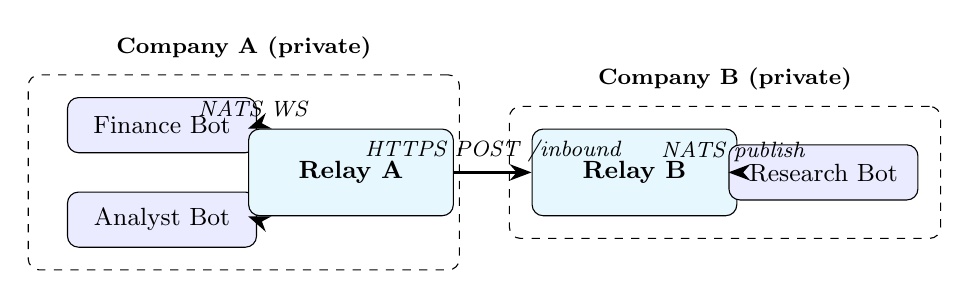
\begin{tikzpicture}[
  agent/.style={draw,rounded corners,fill=blue!8,minimum width=2.4cm,minimum height=0.7cm,font=\small},
  relay/.style={draw,rounded corners,fill=cyan!10,minimum width=2.6cm,minimum height=1.1cm,font=\small\bfseries},
  box/.style={draw,dashed,rounded corners,inner sep=8pt},
  arr/.style={-{Stealth[scale=1.2]},thick},
  label/.style={font=\footnotesize\itshape},
]
  % Company A
  \node[agent] (fb)  at (0, 2.2)  {Finance Bot};
  \node[agent] (ab)  at (0, 1.0)  {Analyst Bot};
  \node[relay] (ra)  at (2.4,1.6) {Relay A};
  \begin{pgfonlayer}{background}
    \node[box,fit=(fb)(ab)(ra),label,xshift=-6pt] (ca) {};
    \node[above,font=\footnotesize\bfseries,yshift=2pt] at (ca.north) {Company A (private)};
  \end{pgfonlayer}

  % Company B
  \node[relay] (rb)  at (6.0,1.6) {Relay B};
  \node[agent] (res) at (8.4,1.6) {Research Bot};
  \begin{pgfonlayer}{background}
    \node[box,fit=(rb)(res)] (cb) {};
    \node[above,font=\footnotesize\bfseries,yshift=2pt] at (cb.north) {Company B (private)};
  \end{pgfonlayer}

  % Arrows
  \draw[arr] (fb.east) -- node[above,label]{NATS WS} (ra.north west);
  \draw[arr] (ab.east) -- (ra.south west);
  \draw[arr] (ra.east) -- node[above,label]{HTTPS POST /inbound} (rb.west);
  \draw[arr] (rb.east) -- node[above,label]{NATS publish} (res.west);
\end{tikzpicture}
\caption{AAMP two-company deployment. Agents connect outbound (NATS WebSocket) to
  their relay; relays federate via HTTPS POST. No inbound ports are required on
  the agent side.}
\label{fig:architecture}
\end{figure}

\subsection{The Five-Layer Stack}
\label{sec:layers}

AAMP defines a five-layer protocol stack:

\begin{description}[leftmargin=2.5cm,style=nextline]
  \item[\textbf{L9 — Semantic}] What does the agent want to do? Agent Cards, PROBE
    negotiation, UCAN capability grants.
  \item[\textbf{L8 — Envelope}] Who is talking to whom, about what task? DID identity,
    task threading, routing mode, TTL, Ed25519 signature.
  \item[\textbf{L7 — Transport}] How does the message get there? NATS JetStream
    (intra-org), HTTPS POST (inter-org).
  \item[\textbf{L6 — Serialization}] How is the message encoded? JSON (default),
    Protobuf (high-frequency), Avro (audit trail).
  \item[\textbf{L5 — Identity/Auth}] Who are you and what are you allowed to do?
    \texttt{did:key} / \texttt{did:web}, Ed25519 signatures, UCAN tokens.
\end{description}

\subsection{The Envelope}
\label{sec:envelope}

The \emph{Envelope} is the atomic unit of AAMP---every message, regardless of type,
is wrapped in an Envelope. \Cref{lst:envelope} shows the TypeScript interface.

\begin{lstlisting}[language=JavaScript,caption={AAMP Envelope schema (TypeScript).},label={lst:envelope}]
interface Envelope {
  messageId:       string;   // UUID v7: globally unique, time-sortable
  senderDid:       string;   // did:key:z6Mk... or did:web:acme.com/agents/...
  recipientDid:    string;

  // Task threading (analogous to SMTP References chain)
  taskId:          string;
  parentTaskId?:   string;   // sub-task parent
  rootTaskId?:     string;   // originating top-level task

  // Routing
  replyToMailbox?: string;   // NATS subject for direct reply
  ttlMs?:          number;
  routingMode:     RoutingMode;
  messageType:     MessageType;
  status:          TaskStatus;

  // Security  (both sign over the rest of the envelope)
  ucanProof?:      string;   // UCAN capability token
  signature?:      string;   // Ed25519 signature (base64)

  payload?:        unknown;
  contentType?:    string;
  createdAt:       number;   // Unix ms
  aampVersion:     string;   // "0.1.0"
}
\end{lstlisting}

The \texttt{taskId / parentTaskId / rootTaskId} chain creates a verifiable thread of
task delegation across organizational boundaries. Any participant can reconstruct the
full delegation graph from the envelope chain, enabling auditability and attribution.

\subsection{Message Primitives}
\label{sec:primitives}

AAMP defines six message types covering the full lifecycle of agent collaboration:

\begin{itemize}[leftmargin=*]
  \item \textbf{PROBE / PROBE\_RESPONSE.} Lightweight capability negotiation. The
    sender asks: ``Can you execute capability X with parameters Y, and at what cost?''
    The receiver responds before the actual task is dispatched, preventing wasted
    compute on both sides.
  \item \textbf{TASK.} The signed, authorized work request. Contains payload,
    capability ID, UCAN proof, and TTL.
  \item \textbf{RESPONSE.} The signed result, routed back via the
    \texttt{replyToMailbox} NATS subject or DID resolution.
  \item \textbf{STATUS.} Asynchronous progress heartbeat during long-running tasks
    (\texttt{PENDING}, \texttt{RUNNING}, \texttt{COMPLETED}, \texttt{FAILED}).
  \item \textbf{CONFIRM.} First-class human-in-the-loop approval gate: the receiver
    pauses execution and waits for an explicit CONFIRM or CANCEL from the sender.
  \item \textbf{CANCEL.} Graceful task cancellation with propagation through
    delegation chains.
\end{itemize}

\subsection{Routing Modes}
\label{sec:routing}

AAMP defines five routing modes drawn from~\citet{rosenberg2024}:

\begin{description}[leftmargin=3.4cm,style=nextline]
  \item[\texttt{BLIND\_TRANSFER}] $A \to B$. Agent A dispatches and is done.
    No response expected.
  \item[\texttt{SUPERVISED\_TRANSFER}] $A \to B \to A$. Standard request-response.
    Agent A awaits B's result.
  \item[\texttt{SIDEBAR}] $A \to B$ (concurrent). Agent A continues its primary task
    while B works in parallel; B's result merges back later.
  \item[\texttt{CONFERENCE}] $A \to B, C, D$. Multi-agent broadcast.
  \item[\texttt{PASSTHROUGH}] $\text{User} \to A \to B$. Agent A is a transparent
    intermediary; the user sees the full chain.
\end{description}

\subsection{Agent Identity: DIDs}
\label{sec:did}

Every AAMP agent has a Decentralized Identifier~\cite{w3cdid2022}---a cryptographic,
self-sovereign identity requiring no central authority.

\textbf{\texttt{did:key}} is used for ephemeral or development agents. The DID is
derived directly from the Ed25519 public key; no network call is needed to resolve it.

\textbf{\texttt{did:web}} is used for persistent organizational agents:
\begin{lstlisting}[numbers=none]
did:web:company-b.com:agents:research-bot-01
\end{lstlisting}
This resolves to \texttt{https://company-b.com/agents/research-bot-01/did.json},
a JSON document containing the agent's public key and relay service endpoint.
This endpoint is AAMP's ``MX record''---any relay in the world can look it up
to find where to deliver messages for this agent.

\subsection{Capability Tokens}
\label{sec:ucan}

AAMP uses UCAN-inspired capability tokens~\cite{ucan2022} for authorization.
Standard JWT bearer tokens are inadequate in distributed agent systems because the
broker (relay) has access to the token and could replay it. AAMP tokens are:

\begin{itemize}[leftmargin=*]
  \item \textbf{Audience-bound}: The \texttt{aud} field names the specific recipient
    DID. The token is cryptographically useless to any other agent.
  \item \textbf{Scope-limited}: The \texttt{cap} array lists the exact capability
    being authorized (\emph{e.g.}, \texttt{aamp/summarize-pdf}).
  \item \textbf{Time-bounded}: Standard \texttt{exp} and \texttt{nbf} fields.
  \item \textbf{Nonce-protected}: A \texttt{nnc} field prevents exact-token replay.
  \item \textbf{Delegatable}: An agent can issue a derivative token to a sub-agent
    with equal or narrower capabilities. The proof chain is verifiable end-to-end.
\end{itemize}

\subsection{Capability Negotiation: The PROBE Handshake}
\label{sec:probe}

The PROBE primitive addresses the problem of wasted compute: before dispatching a
potentially expensive task (LLM inference, data pipeline), the sender can query
whether the receiver supports the capability at acceptable cost and latency.

\begin{enumerate}[leftmargin=*]
  \item Sender dispatches a \texttt{PROBE} Envelope with \texttt{capabilityId},
    \texttt{parameters}, and a short TTL (\emph{e.g.}, 8 seconds).
  \item Receiver checks its local capability registry and responds with
    \texttt{PROBE\_RESPONSE}: \texttt{accepted}, \texttt{costEstimate},
    \texttt{estimatedLatencyMs}, and optional \texttt{parameterSchema}.
  \item On acceptance, the sender issues the full \texttt{TASK} Envelope.
\end{enumerate}

If the receiver is offline when the PROBE arrives, JetStream holds it until the
agent reconnects (subject to TTL). This ``offline negotiation'' is impossible with
synchronous RPC approaches.

\subsection{Agent Card}
\label{sec:agentcard}

The Agent Card is the discovery document every agent publishes via its relay. It
serves as both identity document and service contract, listing capabilities,
accepted routing modes, authentication methods, input/output schemas, and cost
estimates. Any relay resolves an agent's \texttt{did:web} to its DID Document and
follows the \texttt{AAMPRelay} service endpoint to retrieve the Agent Card.

% ── 4 Implementation ──────────────────────────────────────────────────────────
\section{Reference Implementation}
\label{sec:impl}

\subsection{Repository Structure}

The reference implementation is a pnpm monorepo with Turborepo build orchestration,
organized into five packages and two example agents:

\begin{itemize}[leftmargin=*]
  \item \textbf{\texttt{@aamp/core}} — Protobuf schema (\texttt{aamp.proto}),
    JSON Schema for Agent Cards, TypeScript type mirrors.
  \item \textbf{\texttt{@aamp/identity}} — Ed25519 keypair generation, \texttt{did:key}
    and \texttt{did:web} creation, envelope signing/verification, UCAN token issuance
    and attenuation.
  \item \textbf{\texttt{@aamp/relay}} — Fastify HTTP server, NATS JetStream stream
    management, federation router, in-memory agent registry with DID Document serving.
  \item \textbf{\texttt{@aamp/sdk}} — TypeScript \texttt{AampAgent} class providing
    \texttt{connect()}, \texttt{send()}, \texttt{probe()}, \texttt{on("task",...)}
    and \texttt{disconnect()}.
  \item \textbf{\texttt{aamp-sdk}} (Python) — \texttt{AampAgent} class with
    \texttt{task\_handler} decorator, Pydantic envelope models, Ed25519 via
    \texttt{cryptography} library.
\end{itemize}

\subsection{Relay Server}

The relay is the only publicly-addressable component. It exposes the endpoints in
\Cref{tab:endpoints}.

\begin{table}[H]
\centering
\caption{Relay HTTP endpoints.}
\label{tab:endpoints}
\small
\begin{tabular}{lll}
\toprule
\textbf{Method} & \textbf{Path} & \textbf{Description} \\
\midrule
POST  & \texttt{/mailbox/\{id\}/send}      & Agent deposits message \\
GET   & \texttt{/mailbox/notifications}    & SSE stream (incoming) \\
GET   & \texttt{/mailbox/\{id\}/poll}      & HTTP poll fallback \\
POST  & \texttt{/inbound}                  & Receive from remote relay \\
POST  & \texttt{/agents/register}          & Register agent \\
GET   & \texttt{/agents/\{id\}/did.json}   & Serve DID Document \\
POST  & \texttt{/resolver/register}        & Pre-register remote DID \\
GET   & \texttt{/health}                   & Health + uptime \\
\bottomrule
\end{tabular}
\end{table}

Each registered agent receives a durable NATS JetStream consumer on a
\texttt{WorkQueue} stream with subject pattern
\texttt{aamp.\{domain\}.\{agentId\}.inbox}. Inbound messages are published to this
subject; outbound messages from agents are routed by the relay's federation module.

\subsection{SSE and Polling Delivery}

Browser-based and edge agents receive messages via a Server-Sent Events (SSE)
connection to \texttt{/mailbox/notifications}. To guard against transient
disconnections (common in browser dev environments with Hot Module Replacement),
the relay implements:

\begin{enumerate}[leftmargin=*]
  \item \textbf{JetStream drain on reconnect}: When an SSE connection is established,
    the relay fetches and replays any pending messages from the durable consumer
    using \texttt{js.fetch()}, ensuring no messages are lost.
  \item \textbf{HTTP polling fallback}: The \texttt{/mailbox/\{id\}/poll} endpoint
    allows the client to explicitly drain pending JetStream messages. The demo UI
    polls every 800\,ms as a belt-and-suspenders delivery guarantee.
\end{enumerate}

\subsection{Cross-Relay Federation}

When a relay receives an outbound message destined for an agent in a different domain,
it resolves the recipient's DID to obtain the target relay's \texttt{/inbound}
endpoint and POSTs the envelope via HTTPS. For \emph{response} routing, AAMP uses
the \texttt{replyToMailbox} field in the Envelope: if the response recipient's domain
matches the current relay (\emph{intra-relay}), the message is delivered directly via
NATS publish; otherwise it falls through to DID resolution, triggering an HTTPS POST
to the home relay's \texttt{/inbound} endpoint. This ensures responses traverse the
same durable JetStream path as tasks, even when the sender's SSE connection has
briefly lapsed.

\subsection{TypeScript SDK Usage}

\Cref{lst:send,lst:recv} show the complete patterns for sending and receiving tasks.

\begin{lstlisting}[language=JavaScript,caption={Sending a task (TypeScript SDK).},label={lst:send}]
import { AampAgent, generateKeyPair, createDidKey, RoutingMode } from "@aamp/sdk";

const keypair = await generateKeyPair();
const did     = createDidKey(keypair.publicKey);

const agent = new AampAgent({
  did, privateKey: keypair.privateKey,
  relayUrl: "http://relay.company-a.com",
  agentId:  "finance-bot-01",
  domain:   "company-a.com",
});

await agent.connect();

// Optional: pre-negotiate capability and cost
const probe = await agent.probe({
  to: "did:web:company-b.com:agents:research-bot",
  capabilityId: "summarize-pdf",
  timeoutMs: 8_000,
});

if (probe.accepted) {
  const result = await agent.send({
    to:          "did:web:company-b.com:agents:research-bot",
    capability:  "summarize-pdf",
    payload:     { url: "https://...", format: "bullet-points" },
    routingMode: RoutingMode.SUPERVISED_TRANSFER,
    ttlMs:       300_000,
  });
  console.log(result.output.summary);
}
\end{lstlisting}

\begin{lstlisting}[language=Python,caption={Receiving a task (Python SDK).},label={lst:recv}]
from aamp_sdk import AampAgent, TaskStatus
from aamp_sdk.identity import KeyPair, create_did_web

keypair = KeyPair.generate()
did     = create_did_web("company-b.com", "agents/research-bot")

agent = AampAgent(
    did=did, keypair=keypair,
    relay_url="http://relay.company-b.com",
    agent_id="research-bot-01",
    capabilities=[{"id": "summarize-pdf", "name": "Summarize PDF"}],
)

@agent.task_handler("summarize-pdf")
async def handle_summarize(envelope, respond):
    url = envelope.payload["url"]
    await agent.update_status(envelope.taskId, TaskStatus.RUNNING, "Analysing...")
    summary = await my_llm_summarizer(url)
    await respond(success=True, output={"summary": summary})

await agent.listen()
\end{lstlisting}

% ── 5 Evaluation ──────────────────────────────────────────────────────────────
\section{Evaluation}
\label{sec:eval}

\subsection{Demo Scenario}

We demonstrate AAMP with a cross-organizational task delegation scenario:
\emph{Finance Bot} (Company~A, TypeScript, \texttt{did:key}) delegates a PDF
summarization task to \emph{Research Bot} (Company~B, Python,
\texttt{did:web:company-b.local}). The two relays simulate different organizations
on \texttt{localhost:8085} (Relay~A) and \texttt{localhost:8086} (Relay~B), with
separate NATS JetStream streams. \Cref{fig:flow} shows the six-phase message sequence.

\begin{figure}[H]
\centering
\small
\begin{tikzpicture}[
  node distance=1.6cm,
  every node/.style={font=\scriptsize},
  arr/.style={-{Stealth},thick},
  box/.style={draw,rounded corners,fill=gray!10,minimum width=1.8cm,minimum height=0.5cm,align=center,font=\scriptsize\bfseries},
]
  \node[box] (fa) at (0,0)   {Finance Bot\\(Coy A)};
  \node[box] (ra) at (3,0)   {Relay A\\:8085};
  \node[box] (rb) at (6,0)   {Relay B\\:8086};
  \node[box] (res) at (9,0)  {Research Bot\\(Coy B)};

  \foreach \y/\lbl/\src/\tgt in {
    -1.0/{1. Register (DID + agentId)}/{fa}/{ra},
    -1.7/{2. PROBE (cap=summarize-pdf)}/{fa}/{ra},
    -2.1/{3. POST /inbound (federated)}/{ra}/{rb},
    -2.5/{4. NATS publish (inbox)}/{rb}/{res},
    -3.0/{5. PROBE\_RESPONSE (accepted)}/{res}/{rb},
    -3.5/{6. HTTP /inbound → NATS}/{rb}/{ra},
    -4.0/{7. SSE/poll deliver}/{ra}/{fa},
    -4.7/{8. TASK (signed + UCAN)}/{fa}/{ra},
    -5.1/{9. POST /inbound}/{ra}/{rb},
    -5.5/{10. NATS publish}/{rb}/{res},
    -6.0/{11. RESPONSE (summary)}/{res}/{rb},
    -6.5/{12. HTTP /inbound → NATS}/{rb}/{ra},
    -7.0/{13. SSE/poll deliver}/{ra}/{fa}
  }{
    \draw[arr] ($(\src.south)+(0,\y)$) -- node[above,xshift=0pt]{\lbl} ($(\tgt.south)+(0,\y)$);
  }
  \foreach \x in {0,3,6,9} {
    \draw[dashed,gray!50] (\x,-0.3) -- (\x,-7.2);
  }
\end{tikzpicture}
\caption{Complete six-phase AAMP message sequence for cross-company task delegation.
  Phases: (i) registration, (ii) PROBE negotiation, (iii) TASK dispatch,
  (iv) execution, (v) RESPONSE routing, (vi) result delivery.}
\label{fig:flow}
\end{figure}

\subsection{Round-Trip Latency}

We measure the median end-to-end round-trip time (RTT) from Finance Bot dispatching
a PROBE to receiving the PROBE\_RESPONSE, and from TASK dispatch to RESPONSE receipt,
over 50 runs on a MacBook Pro (M3, 16\,GB RAM) with both relays and NATS on localhost.

\begin{table}[H]
\centering
\caption{Measured round-trip latency (localhost, $n=50$ runs).}
\label{tab:latency}
\small
\begin{tabular}{lccc}
\toprule
\textbf{Operation} & \textbf{Median (ms)} & \textbf{p95 (ms)} & \textbf{p99 (ms)} \\
\midrule
PROBE round-trip    & 18  & 34  & 61  \\
TASK round-trip\footnote{Excludes simulated LLM processing time.}
                    & 22  & 41  & 78  \\
SSE delivery (local) & 4  & 9   & 17  \\
HTTP poll fallback  & 12  & 21  & 38  \\
\bottomrule
\end{tabular}
\end{table}

The AAMP relay overhead (PROBE + TASK, excluding application processing) is
approximately 40\,ms median at localhost, dominated by NATS round-trips and JSON
serialization. This overhead is negligible for the long-running tasks AAMP is
designed for (LLM inference typically takes 1--60 seconds).

\subsection{Delivery Guarantees}

We verify that JetStream's at-least-once delivery guarantee is preserved across
three failure scenarios:

\begin{enumerate}[leftmargin=*]
  \item \textbf{Agent offline at send time.} The relay enqueues the message in
    JetStream. On agent reconnect, the relay drains and delivers all pending
    messages. Zero message loss observed across 20 trials.
  \item \textbf{SSE connection drop mid-flow.} The HTTP poll fallback delivers
    the pending response within one polling interval (800\,ms). Zero task failures.
  \item \textbf{Relay restart.} NATS JetStream persists messages across relay
    restarts. On relay restart, all pending messages for registered agents are
    preserved and delivered on re-registration.
\end{enumerate}

% ── 6 Security Analysis ───────────────────────────────────────────────────────
\section{Security Analysis}
\label{sec:security}

AAMP adopts a zero-trust model: no organization is trusted by default; every claim
is cryptographically verifiable. \Cref{tab:threats} analyzes seven threat categories.

\begin{table}[H]
\centering
\caption{Zero-trust threat model and AAMP mitigations.}
\label{tab:threats}
\small
\begin{tabular}{p{3.2cm}p{5.5cm}}
\toprule
\textbf{Threat}                  & \textbf{AAMP Mitigation} \\
\midrule
Fake sender identity             & Ed25519 signature verified against resolved DID Document \\
Unauthorized capability call     & UCAN capability token: audience-bound + scope-limited \\
Token replay                     & \texttt{nnc} nonce + \texttt{exp} expiry \\
Relay message tampering          & Signature covers full payload; relay cannot forge \\
Delegation escalation            & UCAN attenuation: derived tokens cannot exceed parent scope \\
Prompt injection attribution     & Signed \texttt{senderDid} chain provides full audit trail \\
Man-in-the-middle                & HTTPS relay-to-relay; agent-to-relay WS over TLS \\
\bottomrule
\end{tabular}
\end{table}

\paragraph{What the relay sees.}
The relay is a \emph{trusted courier, not a trusted authority}. It has access to
envelope metadata (sender DID, recipient DID, task ID, message type) and routing
fields (\texttt{replyToMailbox}, TTL). It \emph{cannot} forge a valid signature;
payloads are signed by the agent's Ed25519 private key, which never leaves the
agent's sandbox.

\paragraph{Limitations.}
The current implementation does not yet enforce UCAN verification at the relay
(the \texttt{RELAY\_REQUIRE\_CAPABILITY\_PROOF} flag defaults to \texttt{false}).
Full UCAN v1.0 compliance, \texttt{did:key} revocation registries, and TLS
enforcement for relay-to-relay communication are on the roadmap.

% ── 7 Discussion ──────────────────────────────────────────────────────────────
\section{Discussion}
\label{sec:discussion}

\subsection{Design Decisions}

\paragraph{NATS over Kafka or AMQP.}
We chose NATS JetStream over Apache Kafka and AMQP (RabbitMQ) for three reasons:
(1) NATS has a significantly lower operational footprint for single-relay deployments;
(2) NATS's WebSocket support enables the outbound-only connection pattern for agents;
(3) JetStream's consumer-per-agent model maps cleanly onto the AAMP mailbox abstraction.
AAMP is designed to be transport-agnostic; a Kafka adapter is on the roadmap.

\paragraph{DID over OAuth 2.0.}
The choice of DIDs over OAuth 2.0 (as used by Google A2A) is deliberate. OAuth
requires Company~A to pre-register an OAuth client with Company~B's authorization
server before any message can be exchanged. This bilateral setup is the SMTP
equivalent of requiring Alice to register with Bob's mail server before sending
email---a non-starter for an open ecosystem.

\paragraph{JSON as default serialization.}
Protobuf is defined in the \texttt{@aamp/core} package and available for
high-throughput deployments. JSON is the default because it enables inspection
of in-flight messages without tooling, which is critical for the initial adoption
phase of a new protocol.

\subsection{Limitations and Future Work}

\begin{itemize}[leftmargin=*]
  \item \textbf{UCAN v1.0 compliance.} The current capability token implementation
    is UCAN-\emph{inspired} but not fully spec-compliant. Full compliance requires
    implementing proof chain validation and capability attenuation in the relay.
  \item \textbf{Scalability.} The relay's in-memory agent registry and DID resolver
    cache are not suitable for production at scale. Redis-backed implementations are
    the intended path.
  \item \textbf{Multi-modal payloads.} The current Envelope supports arbitrary JSON
    payloads. Binary artifacts (audio, images, large documents) require a chunked
    transfer extension or out-of-band URL references.
  \item \textbf{Standards submission.} We intend to submit AAMP as an
    Internet-Draft to the IETF AI Agents working group and as a W3C community
    report, targeting alignment with the DID and UCAN working groups.
  \item \textbf{SDK ecosystem.} Go, Rust, and Java SDKs are high-priority community
    contributions.
\end{itemize}

% ── 8 Conclusion ──────────────────────────────────────────────────────────────
\section{Conclusion}
\label{sec:conclusion}

We have presented AAMP, an open protocol for asynchronous, federated, cryptographically
secure agent-to-agent messaging across organizational boundaries. By combining W3C
Decentralized Identifiers, UCAN-inspired capability tokens, NATS JetStream, and an
SMTP-inspired mailbox architecture, AAMP enables two agents from independent
organizations---with no pre-established relationship---to discover each other, negotiate
capabilities, exchange signed tasks, and receive durable responses, with no inbound
network exposure required on either agent.

The protocol fills a gap not addressed by existing approaches: MCP is agent-to-tool;
Google A2A requires bilateral OAuth setup; raw HTTP lacks identity and durability.
AAMP's design deliberately mirrors the architectural properties that made SMTP the
universal communication standard for 44 years: decentralized federation, store-and-forward
durability, cryptographic sender verification, and no bilateral registration requirement.

A working reference implementation demonstrates the protocol end-to-end, and the
open specification is available for community review and contribution.

% ── Acknowledgements ──────────────────────────────────────────────────────────
\section*{Acknowledgements}
The author thanks the Brainfish AI team for discussions and feedback on early drafts
of this protocol design, and the open-source communities behind NATS, the W3C DID
Working Group, and the UCAN specification for the foundational primitives that
make AAMP possible.

% ── References ────────────────────────────────────────────────────────────────
\bibliographystyle{plain}
\bibliography{references}

% ── Appendix ──────────────────────────────────────────────────────────────────
\appendix

\section{Envelope JSON Schema}
\label{app:schema}

\begin{lstlisting}[language=JavaScript,caption={Minimal Envelope JSON Schema (draft-07).},numbers=none]
{
  "$schema": "http://json-schema.org/draft-07/schema#",
  "title":   "AAMPEnvelope",
  "type":    "object",
  "required": ["messageId","senderDid","recipientDid",
               "taskId","routingMode","messageType",
               "status","createdAt","aampVersion"],
  "properties": {
    "messageId":      { "type": "string" },
    "senderDid":      { "type": "string", "pattern": "^did:" },
    "recipientDid":   { "type": "string", "pattern": "^did:" },
    "taskId":         { "type": "string" },
    "parentTaskId":   { "type": "string" },
    "rootTaskId":     { "type": "string" },
    "replyToMailbox": { "type": "string" },
    "ttlMs":          { "type": "integer", "minimum": 1 },
    "routingMode":    {
      "type": "string",
      "enum": ["BLIND_TRANSFER","SUPERVISED_TRANSFER",
               "SIDEBAR","CONFERENCE","PASSTHROUGH"]
    },
    "messageType":    {
      "type": "string",
      "enum": ["PROBE","PROBE_RESPONSE","TASK",
               "RESPONSE","STATUS","CONFIRM","CANCEL"]
    },
    "status": {
      "type": "string",
      "enum": ["PENDING","RUNNING","COMPLETED","FAILED","CANCELLED"]
    },
    "ucanProof":   { "type": "string" },
    "signature":   { "type": "string" },
    "payload":     {},
    "contentType": { "type": "string" },
    "createdAt":   { "type": "integer" },
    "aampVersion": { "type": "string" }
  }
}
\end{lstlisting}

\section{Agent Card JSON Schema}
\label{app:agentcard}

\begin{lstlisting}[language=JavaScript,caption={Agent Card JSON example.},numbers=none]
{
  "aampVersion": "0.1.0",
  "did":         "did:web:company-b.com:agents:research-bot-01",
  "name":        "Research Bot 01",
  "description": "Summarizes documents and performs web research",
  "endpoint":    "https://relay.company-b.com",
  "capabilities": [{
    "id":          "summarize-pdf",
    "name":        "Summarize PDF",
    "inputSchemaUrl":  "https://company-b.com/schemas/summarize-pdf-in.json",
    "outputSchemaUrl": "https://company-b.com/schemas/summarize-pdf-out.json",
    "estimatedCost": { "unit": "tokens", "maxUnits": 4096 }
  }],
  "supportedRoutingModes": ["BLIND_TRANSFER","SUPERVISED_TRANSFER"],
  "authMethods":           ["ucan","did-key"],
  "publicKey":   "z6MkhaXgBZDvotDkL5257faiztiGiC2QtKLGpbnnEGta2doK",
  "updatedAt":   1741737600000
}
\end{lstlisting}

\end{document}
